%!TEX root = ../main.tex
% chktex-file 46
\chapter{Learning to Decompose Graphs}%
\label{sec:ltd}

In the last chapter we saw how existing \ac{gcr} approaches relate to \ac{lta}.
Despite their differences, all described \ac{lta} formulations have one thing in common:
Their decomposition functions $\psi$ all split a given graph $G$ into constituents spanned by \ac{bfs} subtrees of $G$ or simply into connected components of $G$.
The only exception to this is the \ac{lta} formulation of \acp{svm} that use fingerprint embeddings; there the constituents are all isomorphic to handpicked substructures.

Apart from the fingerprint embedding approach, which requires domain knowledge in order to pick meaningful substructure patterns, current \ac{gcr} approaches use constituents that are at-best \textit{localized} but not necessarily \textit{interpretable}.
The defining characteristic of \ac{lta} proposed in \cref{sec:ltag:definition}, \textit{localized explainability}, is therefore only partially satisfied by existing approaches.
This shortcoming of the existing \ac{lta} formulations for structured input data gives rise to a new problem:
\begin{defn}
	The \ac{ltd} problem is solved by finding a graph decomposition function $\psi: \mathcal{G}_{\mathcal{D}} \to \mathcal{P}(\mathcal{G}_{\mathcal{D}})$ which splits all graphs $G \in \mathcal{G}_{\mathcal{D}}$ from a given domain $\mathcal{D}$ into constituent subgraphs which are individually ``meaningful'' in the domain $\mathcal{D}$.
\end{defn}

As per our definition of \ac{lta} from \cref{sec:ltag:definition}, the quality of an \ac{lta} formulation is determined by its chosen solution for the \ac{ltd} problem.
Since a comprehensive analysis of this problem would be beyond the scope of this thesis, we focus on the relation between \ac{ltd} and \acp{gcnn}.
The goal of this chapter is to answer the following two questions:
\begin{enumerate}
	\item \textit{Can a stack of graph convolution layers learn a decomposition function dynamically instead of using a static subtree decomposition?}
	\item \textit{What could be the foundation for such an ``\acs{ltd}-convolution'' layer?}
\end{enumerate}

We provide an answer to the first question in \cref{sec:ltd:edge-filter} by showing how decomposition functions $\psi$ can be learned via so-called \textit{edge filters} as part of a convolutional \ac{gnn} architecture.
This establishes the connection between the \acs{ltd} problem and graph convolutions on a high level.
Then the second question is tackled in \crefrange{sec:ltd:kgnn-problems}{sec:ltd:wl2gnn-implementation}.
There a novel graph convolution approach is proposed which could serve as a starting point for an \ac{ltd} convolution layer.

\section{Learning Constituents via Edge Filters}%
\label{sec:ltd:edge-filter}

As we saw in \cref{sec:ltag:formulation:gcnn:conv}, the constituents of neighborhood convolutions are spanned by \ac{bfs} trees of depth $T$, where $T$ is the number of convolutional layers.
From this perspective the problem of learning constituents corresponds to learning a pruning operator on the branches of \ac{bfs} trees.
Such a pruning operator filters the edges that are traversed in each \ac{bfs} step.
There are two general edge filtering strategies:
\begin{enumerate}[label={\textbf{\arabic*.}}]
	\item \textbf{Edge prefiltering:}
		Here the edge filtering and convolution operations are performed in independent steps:
		First the edges of a given graph are filtered, then the convolution layers are applied to the filtered graph.
		This so-called \textit{edge prefiltering} strategy is illustrated in \cref{fig:ltd:subtree-filtering}.
		The main advantage of prefiltering is that it allows arbitrary combinations of edge filtering and convolution approaches.
		The main disadvantage is however that the same edges are removed in all \ac{bfs} subtrees.
		This restricts the expressive power of the learned decomposition function as shown in \cref{fig:ltd:dynamic-subtree-filtering}.
	\item \textbf{Dynamic edge filtering:}
		By filtering edges as part of the convolution operation itself, more flexible decompositions can be obtained.
		In the \textit{dynamic edge filtering} strategy the edge filter is part of the convolution operation and decides which neighbors of a given root node should be aggregated.
		Using this strategy a decomposition such as that shown in \cref{fig:ltd:dynamic-subtree-filtering} is learnable.
\end{enumerate}
\begin{figure}[ht]
	\centering
	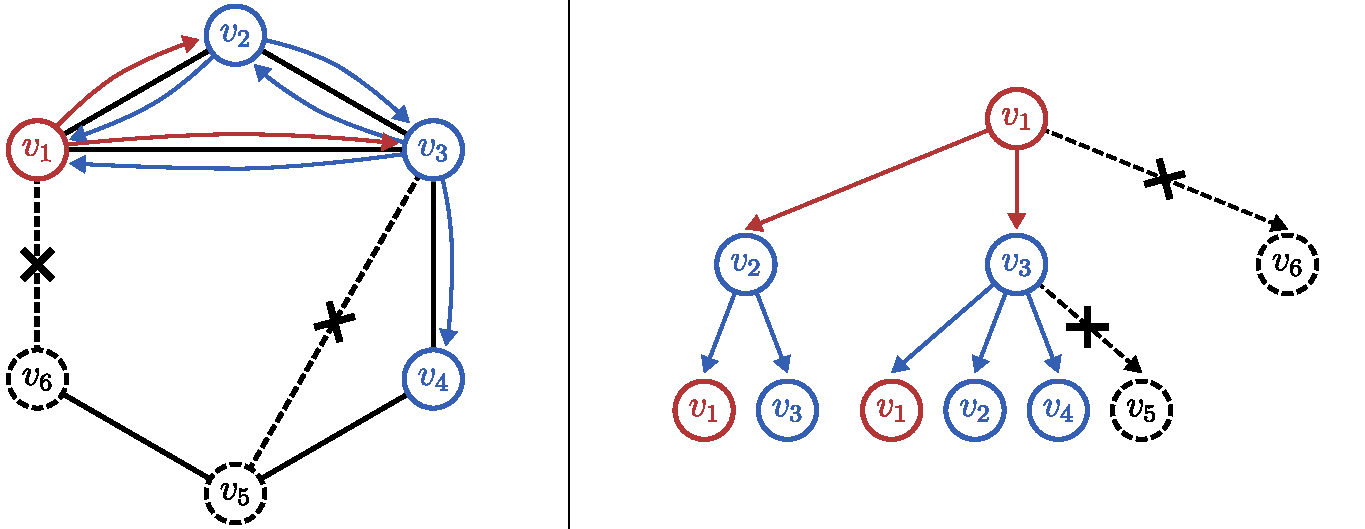
\includegraphics[width=0.8\linewidth]{gfx/ltd/subtree-filtering.pdf}
	\caption{Illustration of a pruned \ac{bfs} subtree when two edges are removed via prefiltering.}\label{fig:ltd:subtree-filtering}
\end{figure}
\begin{figure}[ht]
	\centering
	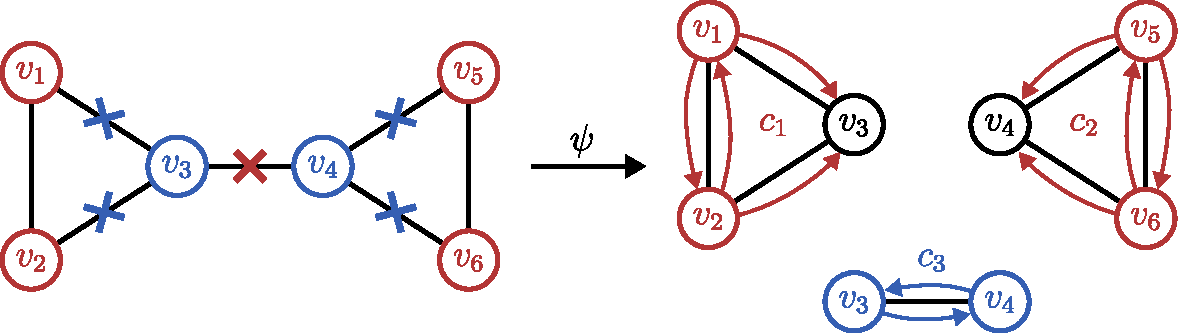
\includegraphics[width=0.75\linewidth]{gfx/ltd/dynamic-subtree-filtering.pdf}
	\caption[A graph decomposition obtained via dynamic edge filtering which cannot be modeled by edge prefiltering.]{
		A graph decomposition obtained via dynamic edge filtering which cannot be modeled by edge prefiltering.
		Depending on the \ac{bfs} root node $v_{\mathrm{root}}$ different edges are removed.
		For $v_{\mathrm{root}} \in \textcolor{t_blue}{\{ v_3, v_4 \}}$ the edges $\{ (v_3, v_1), (v_3, v_2), (v_4, v_5), (v_4, v_6) \}$ are filtered out while for $v_{\mathrm{root}} \in \textcolor{t_red}{\{ v_1, v_2, v_5, v_6 \}}$ the edge $(v_3, v_4)$ is removed. % chktex 25
	}\label{fig:ltd:dynamic-subtree-filtering}
\end{figure}
Irrespective of the chosen edge filtering strategy, the decision whether to remove a given edge $e_{ij} = (v_i, v_j)$ or not has to be made based on relevant information about $e_{ij}$ and its surroundings.
One natural way to encode the information about $e_{ij}$ is via an edge feature vector $z_{ij} \in \mathbb{R}^d$ that is fed into the edge filter.
We propose that those edge feature vectors could be obtained by a 2-\acs{wl} inspired graph convolution layer since 2-\acs{wl} colors represent the structural roles of edges as described in \cref{sec:related:character:wl}.

\section{Shortcomings of the Existing $k$-\acs*{gnn}}%
\label{sec:ltd:kgnn-problems}

\section{The 2-\acs*{wl} Convolution Operator}%
\label{sec:ltd:wl2gnn-definition}

\section{The Expressive Power of 2-\acs*{wl}-\acsp*{gnn}}%
\label{sec:ltd:wl2gnn-properties}

\section{Implementing 2-\acs*{wl}-\acsp*{gnn} on \acsp*{gpgpu}}%
\label{sec:ltd:wl2gnn-implementation}
